\chapter{Rubber Motors}

Rubber in its natural form comes from trees found in places like the Amazon, Indonesia, and others around the world. Chemists have determined that an organic compound found in these trees helpds protect them from temperature fluctuations. The compound is called {\it isoprene} and looks like this when drawn as a chemical figure:

\begin{figure}
    \begin{center}
       \setchemfig{atom sep=18.34pt}
       \chemfig{-[@{a}]CH_{2}-[::-45]C(-[::-90]H_{3}C)(=CH-[::45]CH_{2}-[@{b}])}
       \makepolymerdelims[delimiters={[]}]{5pt}[27pt]{a}{b}  
    \end{center}
    \caption{Natural Rubber: polyisoprene molecule}
\end{figure}

Here is a nice website that has more information about this molecule. \href{https://pslc.ws/macrog/isoprene.htm}.

Natural rubber is stretchy and has properties that were interesting to many folks. However, it had a few deficiencies, so chemists played with this moleculr and discovered that if they heated it up and mixed in some sulfer under high pressure, a process called vulcanization, something interesting happened.

At the molecular level the sulfer caused two polymide submolecules to bone together, effectively connecting two adjacent polymer chains together. Not ever submolecure became linked, just enough to provide new properties.

\begin{figure}[ht]
    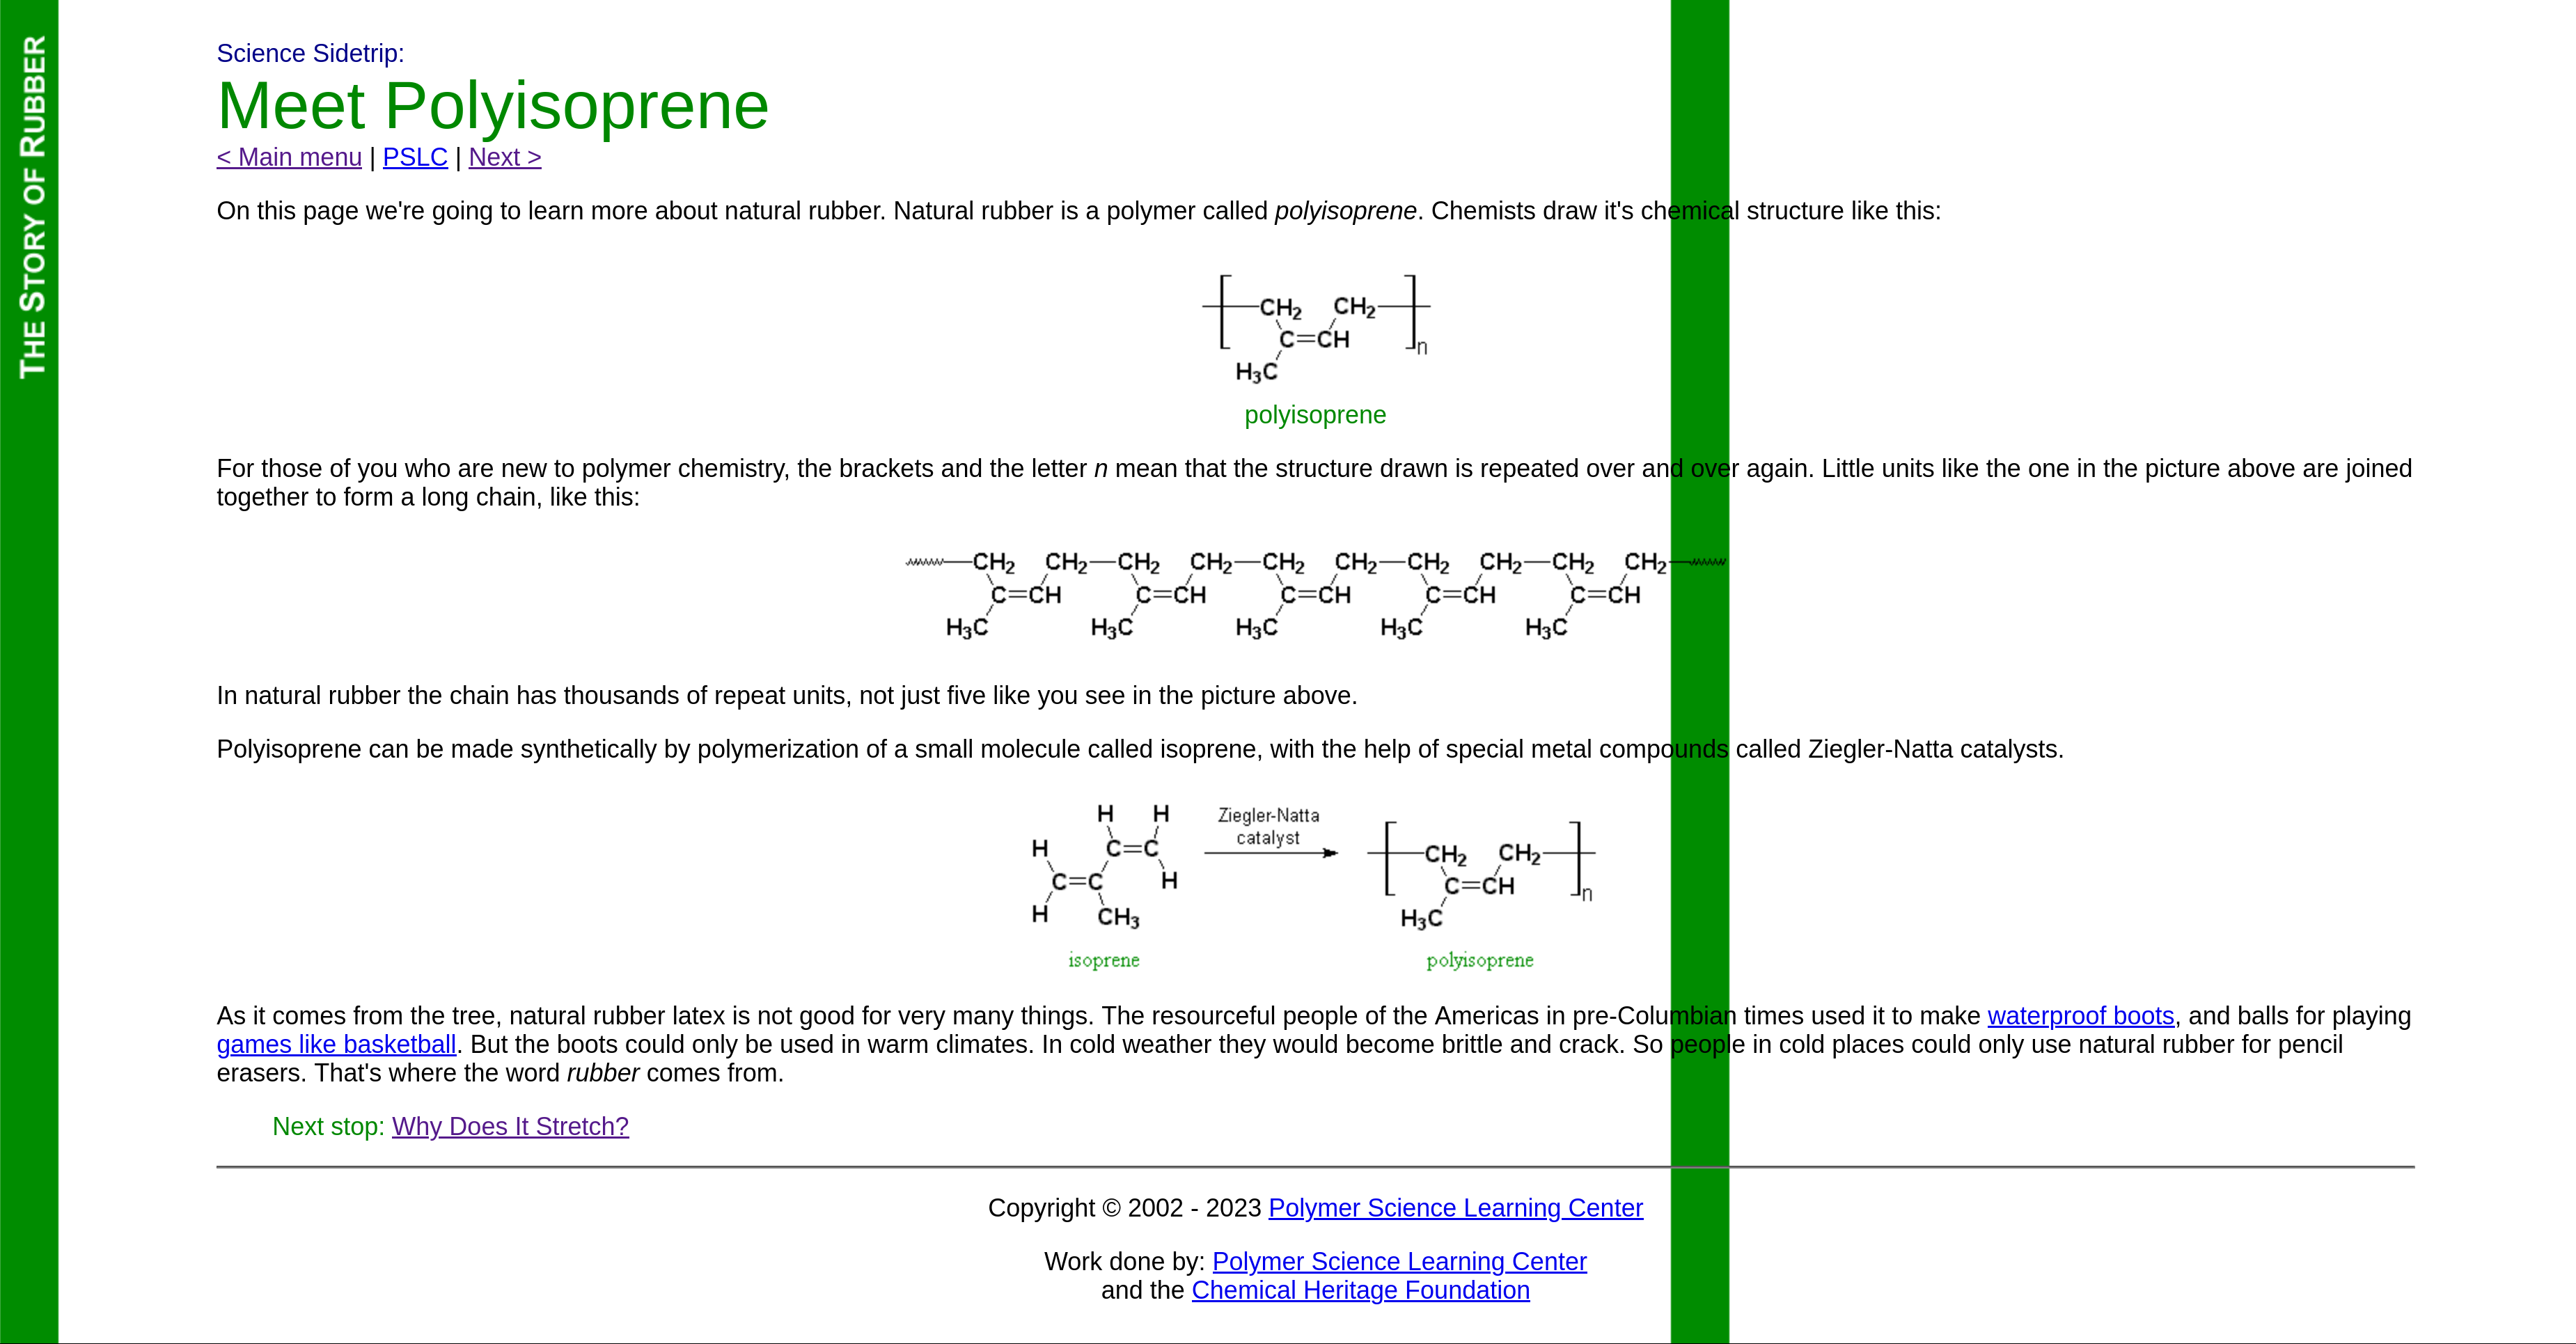
\includegraphics[width=0.7\textwidth]{test.png}
    \centering
    \caption{test figure}
    
\end{figure}

This article needs a reference \cite{maheswaramma:2015}

\begin{figure}[ht]
    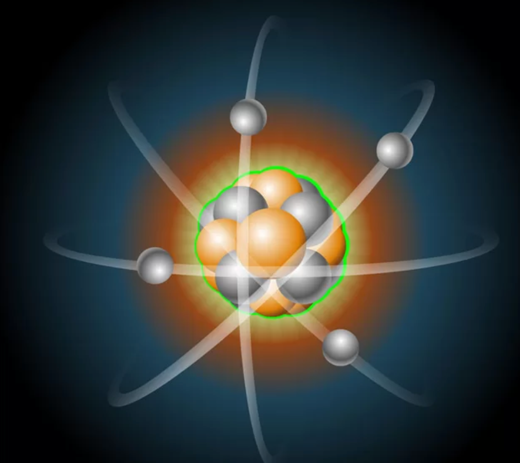
\includegraphics[width=0.7\textwidth]{atomic-structure.png}
    \centering
    \caption{Atomic structure.}
\end{figure}
